%%%%%%%%%%%%%%%%%%%%%%%%%%%%%%%%%%%%%%%%%
% Beamer Presentation
% LaTeX Template
% Version 1.0 (10/11/12)
%
% This template has been downloaded from:
% http://www.LaTeXTemplates.com
%
% License:
% CC BY-NC-SA 3.0 (http://creativecommons.org/licenses/by-nc-sa/3.0/)
%
%%%%%%%%%%%%%%%%%%%%%%%%%%%%%%%%%%%%%%%%%

%----------------------------------------------------------------------------------------
%	PACKAGES AND THEMES
%----------------------------------------------------------------------------------------

\documentclass{beamer}

\usepackage[utf8]{inputenc}
\usepackage[french]{babel}
\usepackage{enumerate}
\usepackage{array,multirow,colortbl}
\usepackage{enumitem}
\usepackage{animate}
\usepackage{graphicx} % Allows including images
\usepackage{booktabs} % Allows the use of \toprule, \midrule and \bottomrule in tables
\usepackage[compatibility=false]{caption}
\usepackage{subcaption}
\usepackage{cite}
\usepackage[numbers]{natbib}
\usepackage[T1]{fontenc}
\usepackage[default]{gillius}
\mode<presentation> {

% The Beamer class comes with a number of default slide themes
% which change the colors and layouts of slides. Below this is a list
% of all the themes, uncomment each in turn to see what they look like.

%\usetheme{default}
%\usetheme{AnnArbor}
%\usetheme{Antibes}
%\usetheme{Bergen}
%\usetheme{Berkeley}
%\usetheme{Berlin}
%\usetheme{Boadilla}
%\usetheme{CambridgeUS}
%\usetheme{Copenhagen}
%\usetheme{Darmstadt}
%\usetheme{Dresden}
%\usetheme{Frankfurt}
%\usetheme{Goettingen}
%\usetheme{Hannover}
%\usetheme{Ilmenau}
%\usetheme{JuanLesPins}
%\usetheme{Luebeck}
%\usetheme{Madrid}
%\usetheme{Malmoe}
%\usetheme{Marburg}
%\usetheme{Montpellier}
%\usetheme{PaloAlto}
%\usetheme{Pittsburgh}
%\usetheme{Rochester}
\usetheme{Singapore}
%\usetheme{Szeged}
%\usetheme{Warsaw}

% As well as themes, the Beamer class has a number of color themes
% for any slide theme. Uncomment each of these in turn to see how it
% changes the colors of your current slide theme.

%\usecolortheme{albatross}
%\usecolortheme{beaver}
%\usecolortheme{beetle}
%\usecolortheme{crane}
%\usecolortheme{dolphin}
%\usecolortheme{dove}
%\usecolortheme{fly}
\usecolortheme{lily}
%\usecolortheme{orchid}
%\usecolortheme{rose}
%\usecolortheme{seagull}
%\usecolortheme{seahorse}
%\usecolortheme{whale}
%\usecolortheme{wolverine}

%\setbeamertemplate{footline} % To remove the footer line in all slides uncomment this line
\setbeamertemplate{footline}[page number] % To replace the footer line in all slides with a simple slide count uncomment this line

\setbeamertemplate{navigation symbols}{} % To remove the navigation symbols from the bottom of all slides uncomment this line
}


%----------------------------------------------------------------------------------------
%	TITLE PAGE
%----------------------------------------------------------------------------------------

\title[PFA 2014-2015]{PFA 2014-2015 \\ \LARGE De la 3D vers la 2D} % The short title appears at the bottom of every slide, the full title is only on the title page

\author{Anaïs BOHER, Yohann CABON, Magali CHAUVAT, Akané LEVY, Thomas MARCELIN, Xavier MAUPEU, Alexandre PHILIPPI
\\ \and \\
\underline{Clients :} Carole BLANC, Pascal DESBARATS 
\\
\underline{Encadrant :} Sylvain LOMBARDY} 

\institute[Enseirb-Matmeca] % Your institution as it will appear on the bottom of every slide, may be shorthand to save space
{École Nationale Supérieure d'Électronique, Informatique, Télécommunications, Mathématiques et Mécanique de Bordeaux
}
\date{} % Date, can be changed to a custom date

\setbeamertemplate{section in head/foot}{\hfill\insertsectionheadnumber.~\insertsectionhead}
\setbeamertemplate{section in head/foot shaded}{\color{structure!50}\hfill\insertsectionheadnumber.~\insertsectionhead}
\setbeamertemplate{section in toc}{ \inserttocsectionnumber.~\inserttocsection}

\begin{document}
\graphicspath{{./images/}{.}}


%------------------------------------------------



\begin{frame}
\titlepage % Print the title page as the first slide

\begin{figure}[B]
\vspace*{-1cm}

\includegraphics[scale=0.4]{logo.png}
\end{figure}
\end{frame}
% % TODO : caption pour les images 

%------------------------------------------------

%plan sur le cote 
%introduction
%cahier des charges 
%implementation
%gestion des projets

%------------------------------------------------
\section{Introduction}
% TODO : INTRO a remplir : THOMAS
% TODO : remplir la slide du contexte
\begin{frame}
\frametitle{Contexte}

\begin{itemize}[label=$\bullet$]
\item Projet proposé par des chercheurs du LaBRI
\item parler du domaine ?
\end{itemize}
\end{frame}

%------------------------------------------------

% %TODO : remplacer par un schéma, les points 
% TODO objectif: représentation d'une scène
%parler des anaglyphes, autostéreogrammes, flipbooks 
%slide 1:  schéma 
% slide d'après : anaglyphes/autostereogrammes/gif/scene

\begin{frame}
\frametitle{Présentation du sujet (1/4)}

\begin{itemize}[label=$\bullet$]
\item Schéma A FAIRE
\end{itemize}
\end{frame}

%------------------------------------------------

% % TODO : MAGALI tu peux vérifier le caption et mettre ce qu'il faut, et remplacer l'image aussi
\begin{frame}

\frametitle{Présentation du sujet (2/4)}

\begin{itemize}[label=$\bullet$]
\item Autostéréogramme
\end{itemize}
\begin{figure}
\centering
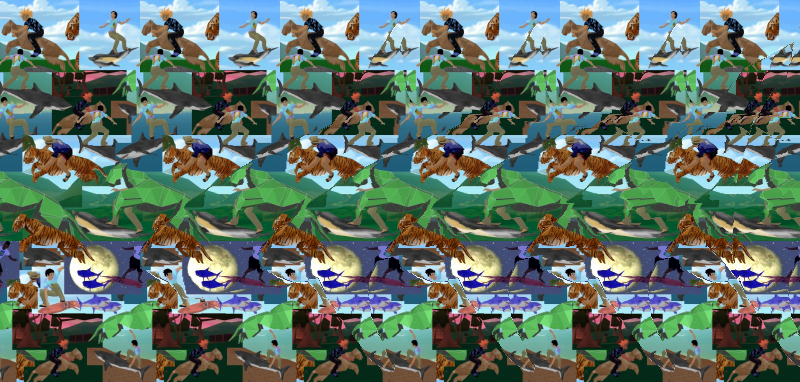
\includegraphics[scale=0.4]{autostereog.png} % de même
\caption{Autostéréogramme d'un requin \footnotemark}
\end{figure}
\footnotetext{\url{http://en.wikipedia.org/wiki/Autostereogram}}

\end{frame}

%------------------------------------------------

\begin{frame}

\frametitle{Présentation du sujet (3/4)}

\begin{itemize}[label=$\bullet$]
\item Anaglyphe
\end{itemize}
\begin{figure}
\centering
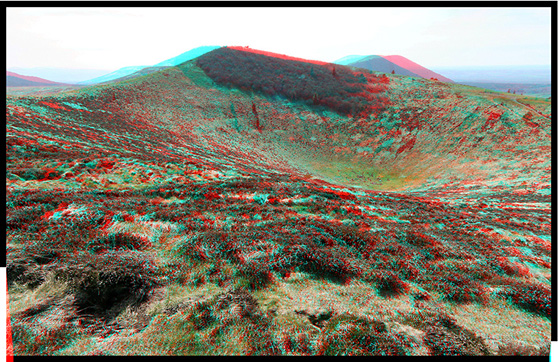
\includegraphics[scale=0.4]{anaglyphe-cratere-puy.jpg} % pas obligé de mettre des donuts
\caption{Anaglyphe d'un paysage \footnotemark}
\end{figure}
\footnotetext{\url{http://www.photo-stereo.com/images/anaglyphe-cratere-puy.jpg}}

\end{frame}

%------------------------------------------------

% % TODO changer par un gif ici, pas obligé de mettre les donuts
% % TODO : faire apparaître le mot "folioscope"


\begin{frame}

\frametitle{Présentation du sujet (4/4)}

\begin{itemize}[label=$\bullet$]
\item Flipbook (folioscope)
\end{itemize}
\begin{figure}
\centering
\animategraphics[autoplay,loop,height=5cm]{1}{gifimages/ex_gif_}{00}{29}
\caption{Animation gif\footnotemark}
\end{figure}
\footnotetext{\url{http://shyrobotics.com/wp-content/uploads/2012/09/Mouvement-precession.gif}}
\end{frame}

%------------------------------------------------
% OK : les besoins en liste 
%
\section{Cahier des charges}


\begin{frame}
\frametitle{Besoins non fonctionnels et contraintes}
\begin{itemize}[label=$\bullet$]
\item Besoins fonctionnels
	\begin{itemize}[label=$\circ$]
	\item Manipulation de la caméra
	\item Manipulation des objets
	\item Sauvegardes et chargement
	\item Anaglyphes, autostéréogrammes, folioscopes
	\end{itemize}
\item Besoins non fonctionnels
	\begin{itemize}[label=$\circ$]
	\item Extensibilité
	\item Portabilité
	\item Fluidité
	\end{itemize}
\end{itemize}
\end{frame}

%------------------------------------------------

\begin{frame}
\frametitle{Architecture (1/3)}
\centering
\begin{figure}
  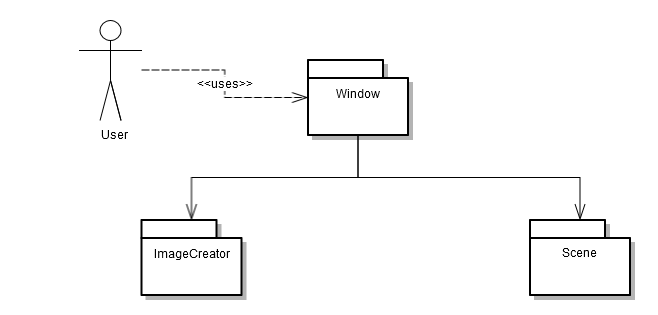
\includegraphics[scale=0.4]{paquetages.jpg}
  \caption{Diagramme des paquetages}
\end{figure}
\end{frame}

%------------------------------------------------

\begin{frame}
\frametitle{Architecture (2/3)}
\centering
\begin{figure}
  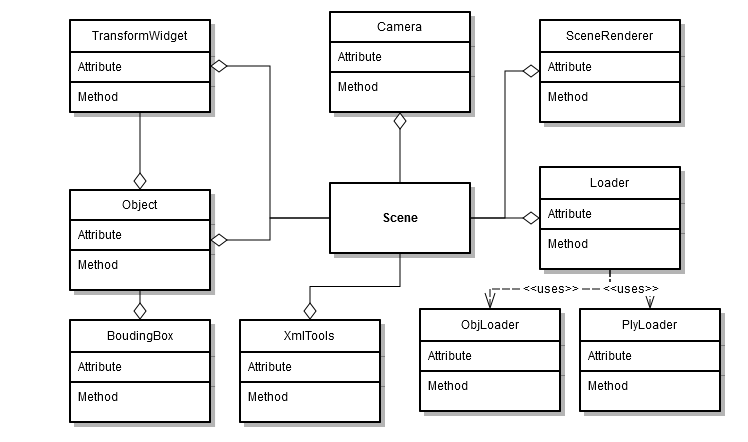
\includegraphics[scale=0.4]{scene.png}
  \caption{Paquetage scène}
\end{figure}
\end{frame}

%------------------------------------------------
% 
% ensuite présenter archi  
% ATTENTION pas de capture d'écran ici
% TODO PHILIPPI : présenter l'architecture qui remplie les besoins du cahier de charge
% du genre classes virtuelles pour l'extensibilité par ex

\begin{frame}
\frametitle{Architecture (3/3)}
\begin{itemize}[label=$\bullet$]
\item Extensibilité : utilisation de classes virtuelles
\end{itemize}
\centering
\begin{figure}
  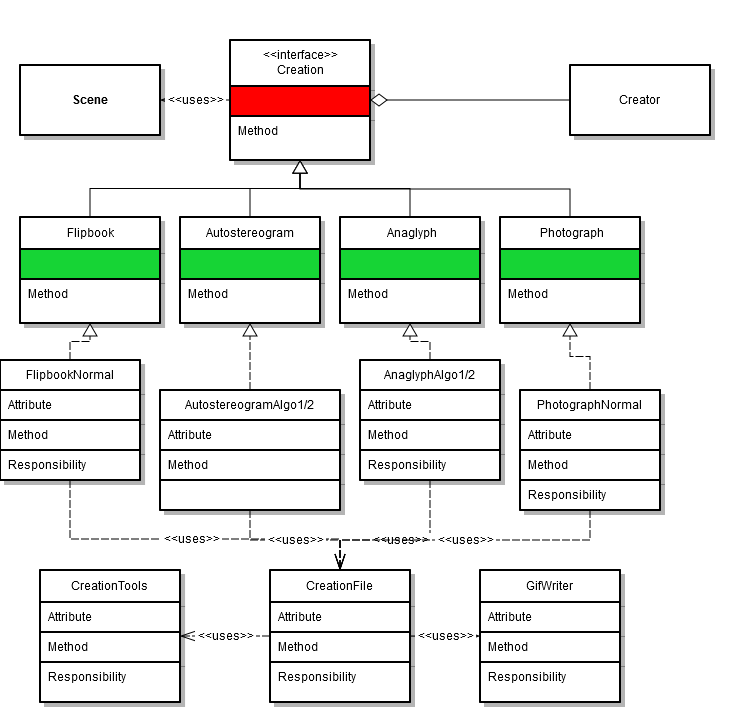
\includegraphics[scale=0.25]{extensibilite.png}
  \caption{Paquetage création}
\end{figure}
\end{frame}

%%------------------------------------------------
% TODO : au début présentation du logiciel, faire une scène 2 tores, en rendu, flipbook, anaglyphes, autostereogrammes, 
% que le résultat

\section{Implémentation}

\begin{frame}
\frametitle{Présentation du logiciel (1/5)}
\begin{figure}
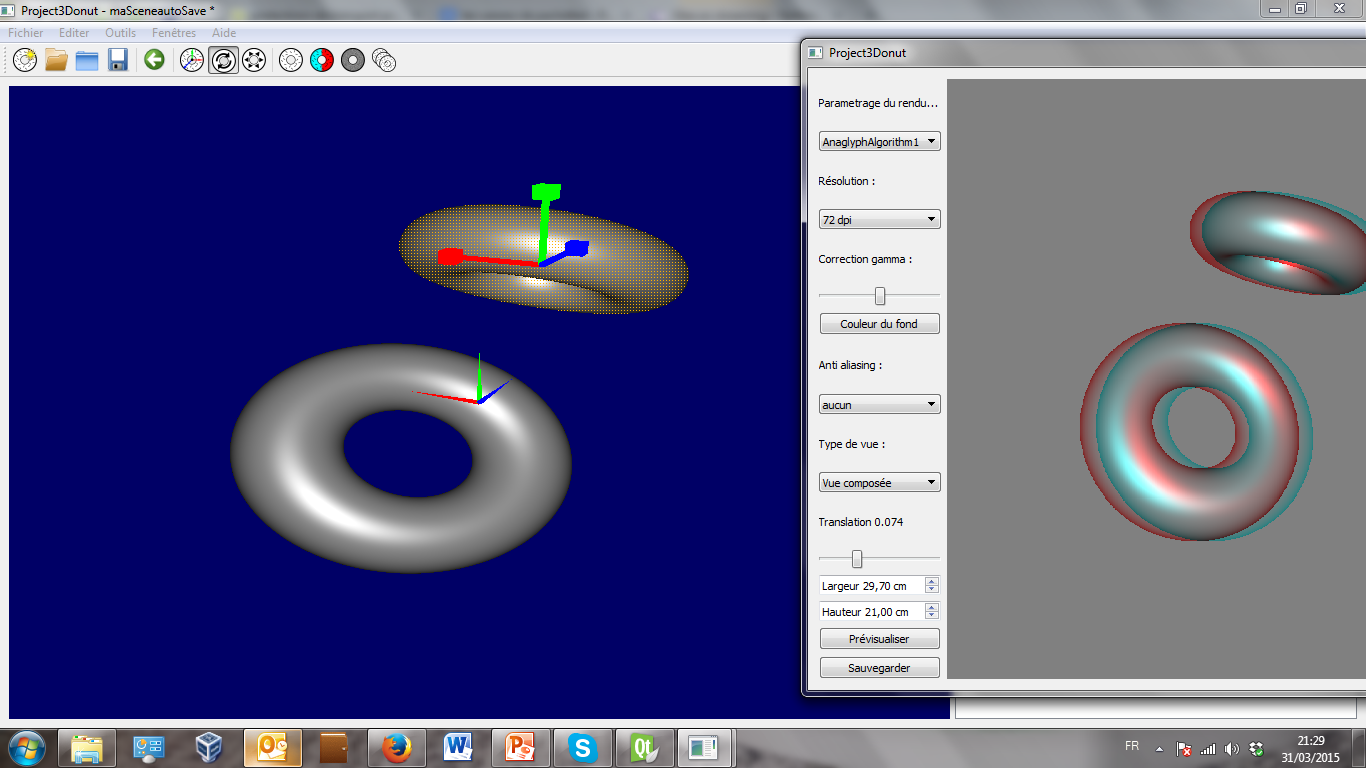
\includegraphics[scale=0.22]{logiciel.png}
\caption{Vue du logiciel}
\end{figure}
\end{frame}
% OK : couper les screens et les remplir
% OK : mettre des sous titres

%%------------------------------------------------
%
% OK : MAGALI screen shot plz
\begin{frame}
\frametitle{Présentation du logiciel (2/5)}
\begin{itemize}[label=$\bullet$]
\item Rendu de la scène
\end{itemize}
\begin{figure}
\centering
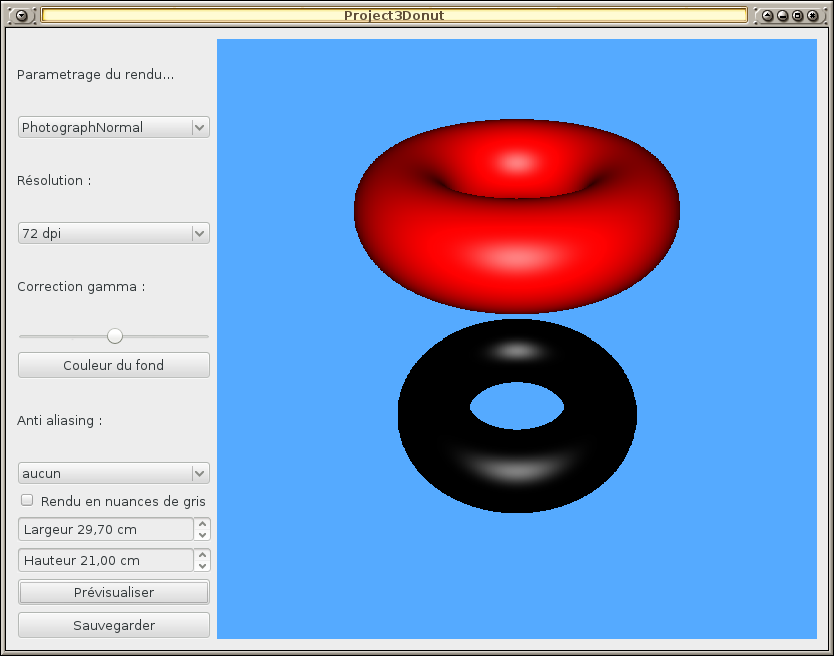
\includegraphics[scale=0.28]{rendu.png}
\caption{Rendu d'une scène contenant deux tores}
\end{figure}

\end{frame}

%%------------------------------------------------
%
\begin{frame}
\frametitle{Présentation du logiciel (3/5)}
\begin{itemize}[label=$\bullet$]
\item Flipbook (folioscope)
\end{itemize}
\begin{figure}
\centering
\animategraphics[autoplay,loop,height=6.5cm]{1}{gifimages/rendu_gif_}{00}{49}
\caption{Gif animé obtenu à partir du logiciel}
\end{figure}
\end{frame}



%%------------------------------------------------
%
% OK : MAGALI screen shot plz
\begin{frame}
\frametitle{Présentation du logiciel (4/5)}
\begin{itemize}[label=$\bullet$]
\item Autostéréogramme
\end{itemize}
\begin{figure}
\centering
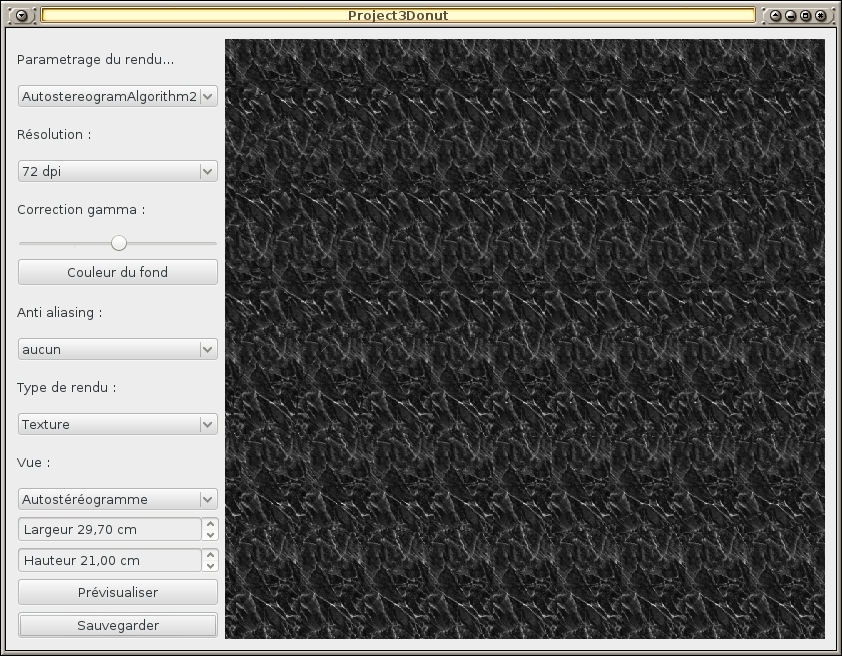
\includegraphics[scale=0.28]{renduautostereogrammes.png}
\caption{Autostéreogramme obtenu à partir du logiciel}
\end{figure}
\end{frame}

%%------------------------------------------------
%
% OK : MAGALI screen shot plz
\begin{frame}
\frametitle{Présentation du logiciel (5/5)}
\begin{itemize}[label=$\bullet$]
\item Anaglyphe
\end{itemize}
\begin{figure}
\centering
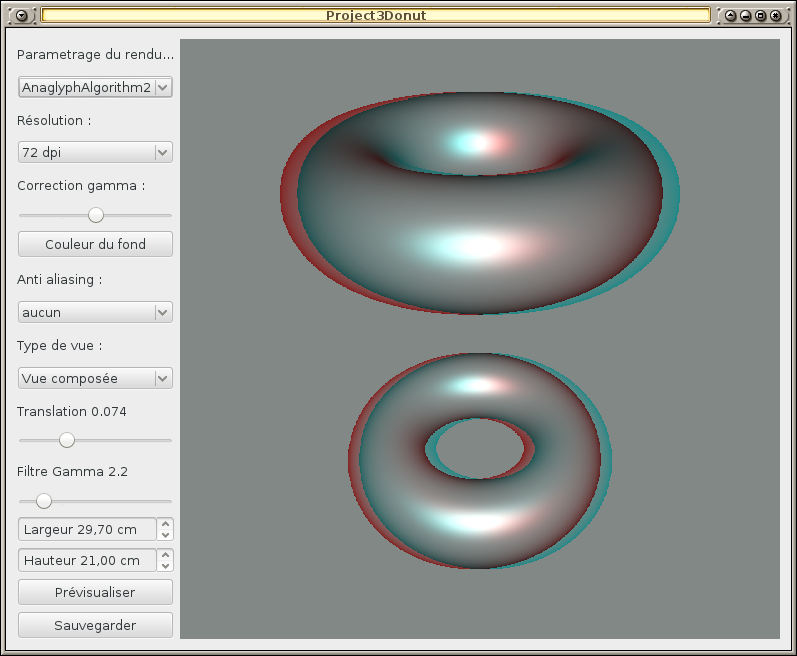
\includegraphics[scale=0.28]{renduanaglyphe.png}
\caption{Anaglyphe obtenu à partir du logiciel}
\end{figure}
\end{frame}

%%------------------------------------------------

% % XAVIER :

\begin{frame}
\frametitle{Choix techniques}
\begin{itemize}[label=$\bullet$]
	\item Utilisation du C++11
	\item Interface graphique avec Qt5
	\item Rendu avec OpenGL
\end{itemize}

\end{frame}

%------------------------------------------------

\begin{frame}
\frametitle{Rendu 2D avec OpenGL}
\begin{figure}
\centering
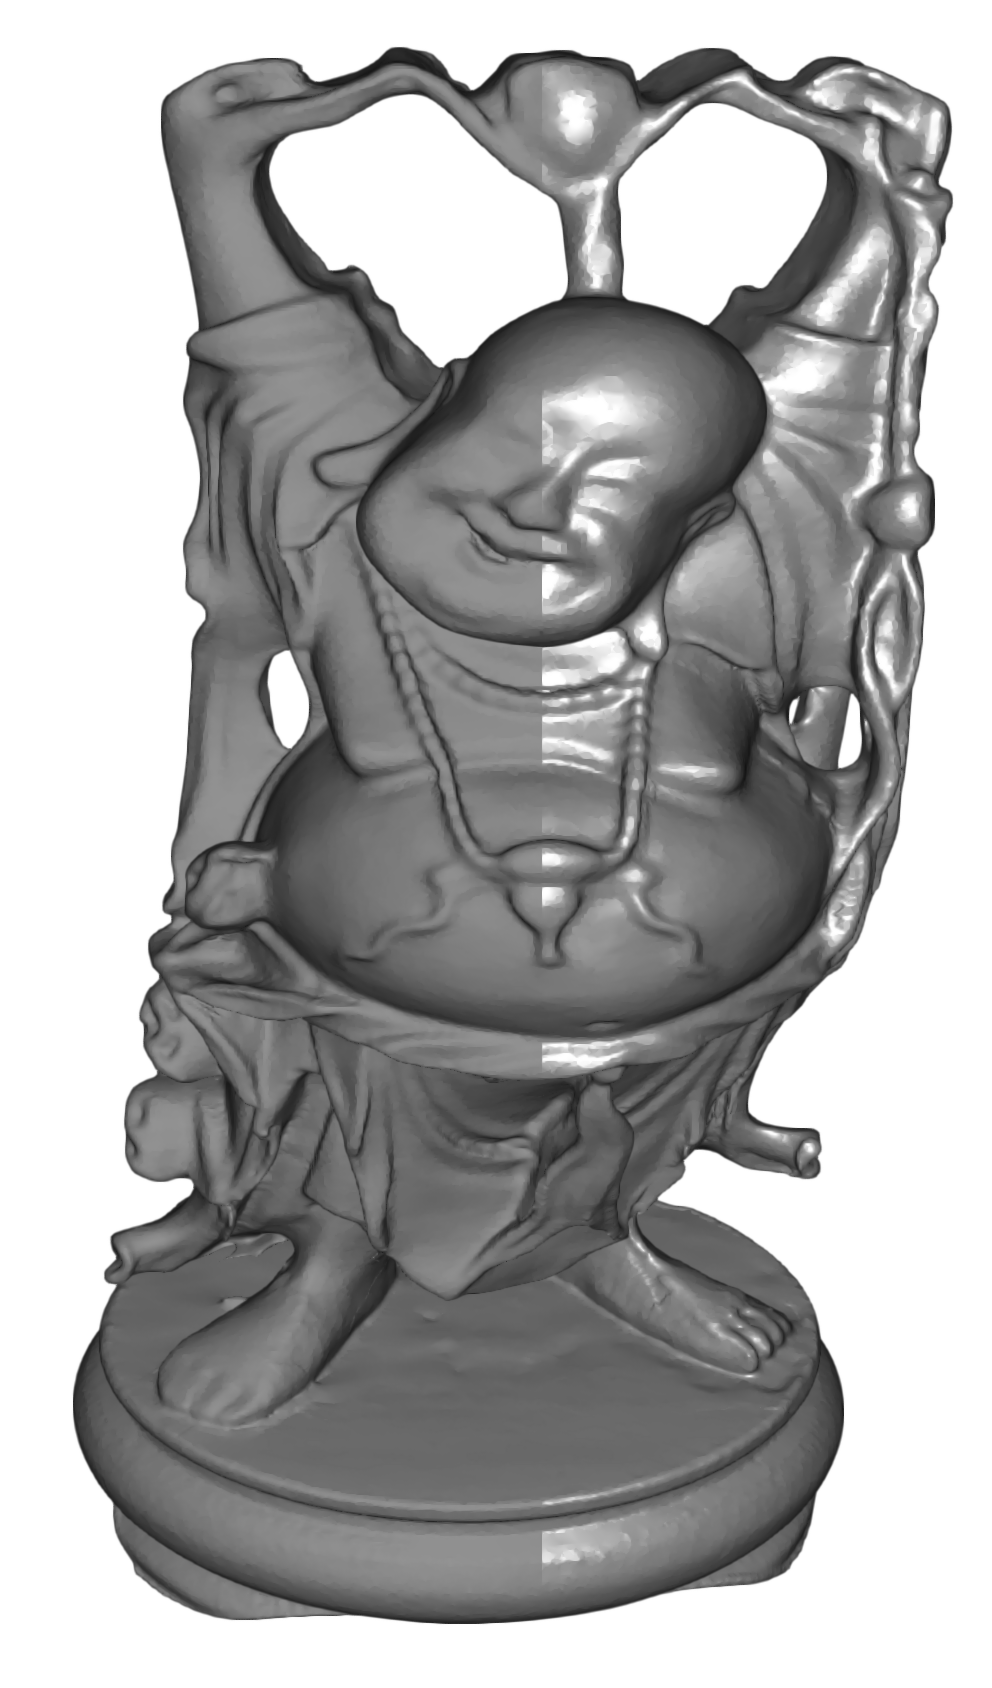
\includegraphics[scale=0.15]{rendu_specular.png}
\caption{Rendu avec et sans spécularité}
\end{figure}

\end{frame}

%------------------------------------------------

\begin{frame}
\frametitle{Anti-aliasing}
\begin{figure}
\centering
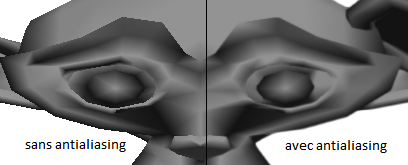
\includegraphics[scale=0.8]{antialiasing.png}
\caption{Rendu avec et sans antialiasing}
\end{figure}

\end{frame}

%------------------------------------------------

%
\begin{frame}
\frametitle{Autostéréogramme (1/3) : principe}

\begin{itemize}[label=$\bullet$]
\item Génération d'une carte de profondeurs
\item Obtention de l'autostéréogramme
\end{itemize}

\begin{figure}
\centering
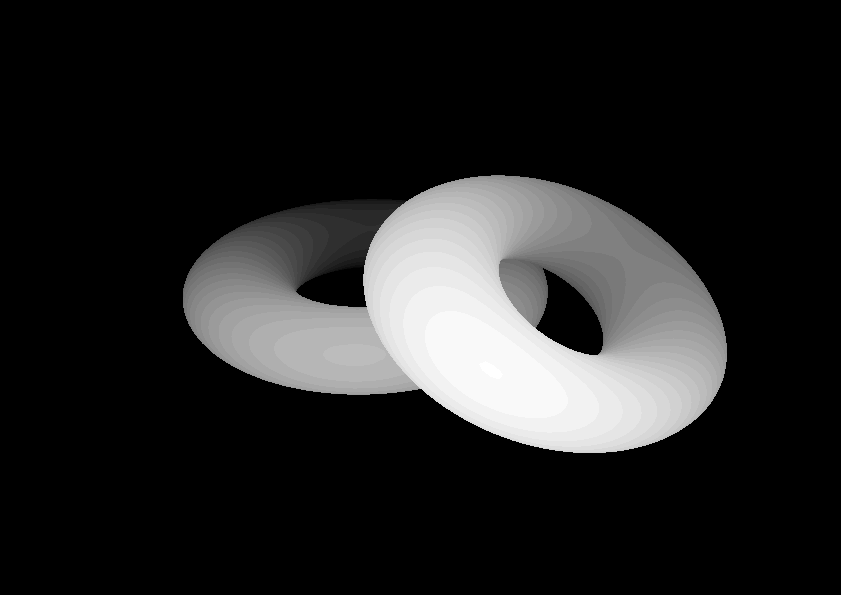
\includegraphics[scale=0.22]{donutdepth.png}
\caption{Carte des profondeurs obtenue avec le logiciel}
\end{figure}
\end{frame}
%%------------------------------------------------
% ORAL : demande une certaine gymnastique de voir les autostéréogrammes
% recherche existant , choix d'implémenter deux pour avoir deux rendus différents
\arrayrulecolor{white}   

\begin{frame}
\frametitle{Autostéréogramme (2/3)}
\begin{itemize}[label=$\bullet$]
\item Algorithme de Thimbelby, Inglis, Witten \cite{stereogram}
	\begin{itemize}[label=$\circ$]
	\item Algorithme ``de base''
	\item Plus adapté aux formes simples et peu détaillés
	\end{itemize}
\end{itemize}
\begin{figure}
\centering
\begin{subfigure}{.4\textwidth}
  \centering
  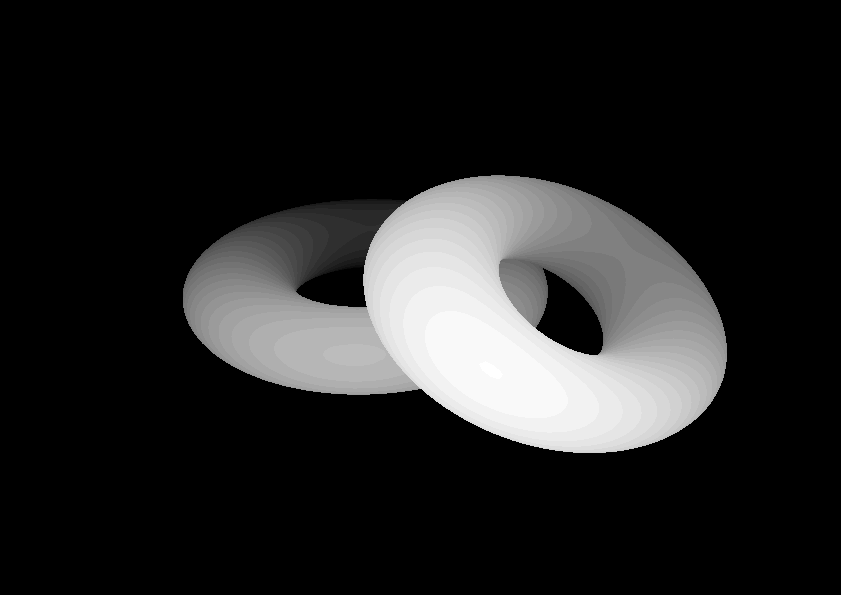
\includegraphics[width=1\linewidth]{donutdepth.png}
  \caption{Carte de profondeurs}
\end{subfigure}
\begin{subfigure}{.4\textwidth}
  \centering
  
\includegraphics[width=1\linewidth]{donut1.png}
  \caption{Autostéréogramme réalisé}
\end{subfigure}
\caption{Résultat obtenu avec l'algorithme de Thimbelby, Inglis, Witten}
\end{figure}


\end{frame}

%%------------------------------------------------
%
% TODO : MAGALI complexite à rajouter
\begin{frame}
\frametitle{Autostéréogramme (3/3)}
\begin{itemize}[label=$\bullet$]
	\item Algorithme de W.A Steer \cite{wasteer}
	\begin{itemize}[label=$\circ$]
	\item Algorithme plus élaboré
	\item Amélioration 3D : suréchantillonage
	\item Amélioration 2D : coloration symétrique
	\item Complexité : $O(mn)$
	\end{itemize}
\end{itemize}
\begin{figure}
\centering
\begin{subfigure}{.4\textwidth}
  \centering
  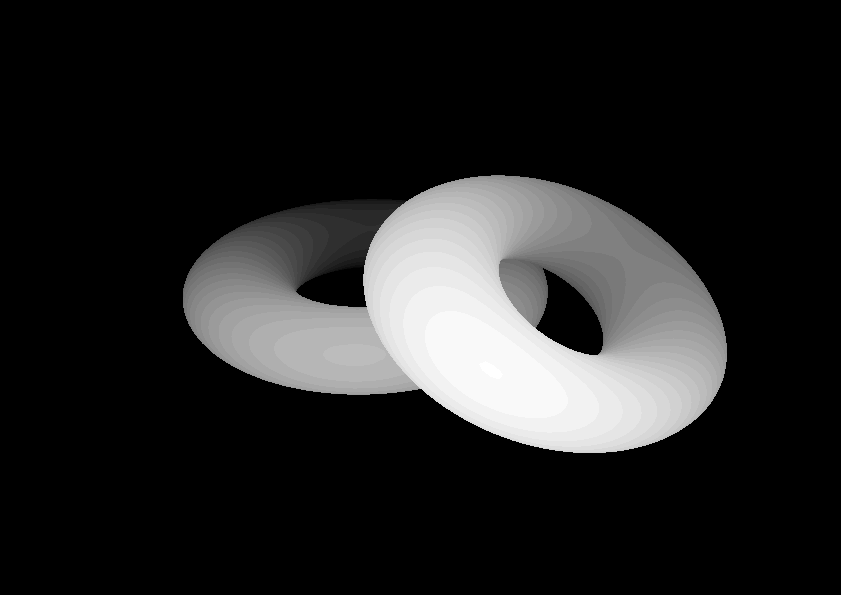
\includegraphics[width=1\linewidth]{donutdepth.png}
  \caption{Carte de profondeurs}
\end{subfigure}
\begin{subfigure}{.4\textwidth}
  \centering
  
\includegraphics[width=1\linewidth]{donut2.png}
  \caption{Autostéréogramme réalisé}
\end{subfigure}
\caption{Résultat obtenu avec l'algorithme de W.A Steer}
\end{figure}
%\begin{tabular}{l|r}
%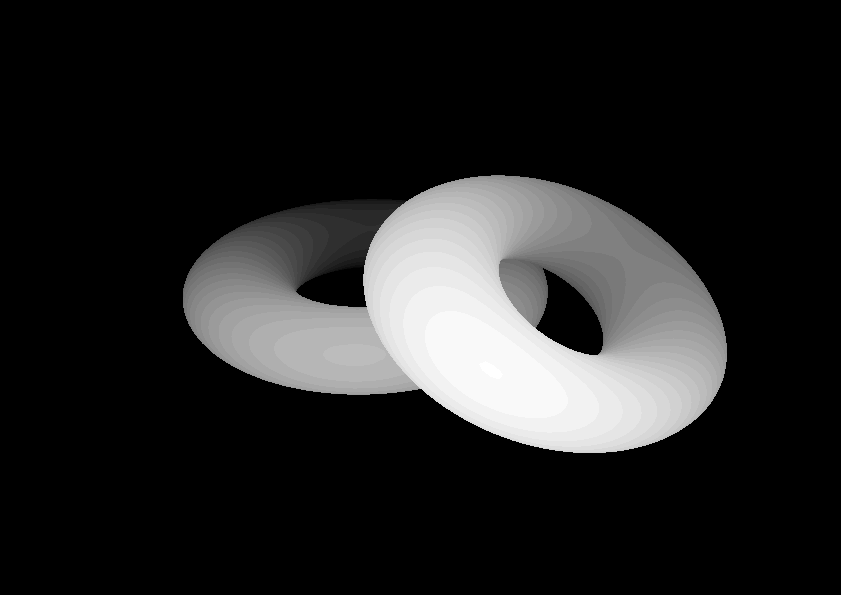
\includegraphics[scale=0.22]{donutdepth.png}
%&
%
\includegraphics[scale=0.22]{donut2.png}
%\end{tabular}

\end{frame}
%%------------------------------------------------

%

% % ORAL : on avait deux images de base on les a pas généré ! 
\begin{frame}
\frametitle{Anaglyphe (1/6)}
\begin{itemize}[label=$\bullet$]
\item Méthode Photoshop \cite{stereoAnaglyph}
	\begin{itemize}[label=$\circ$]
	\item Algorithme ``de base''
	\item Composé de trois étapes 
	\item Première étape : translation de la prise de vue d'une distance proche à celles entre les yeux 
	\end{itemize}
\end{itemize}

\begin{figure}
\centering
\begin{subfigure}{.5\textwidth}
  \centering
  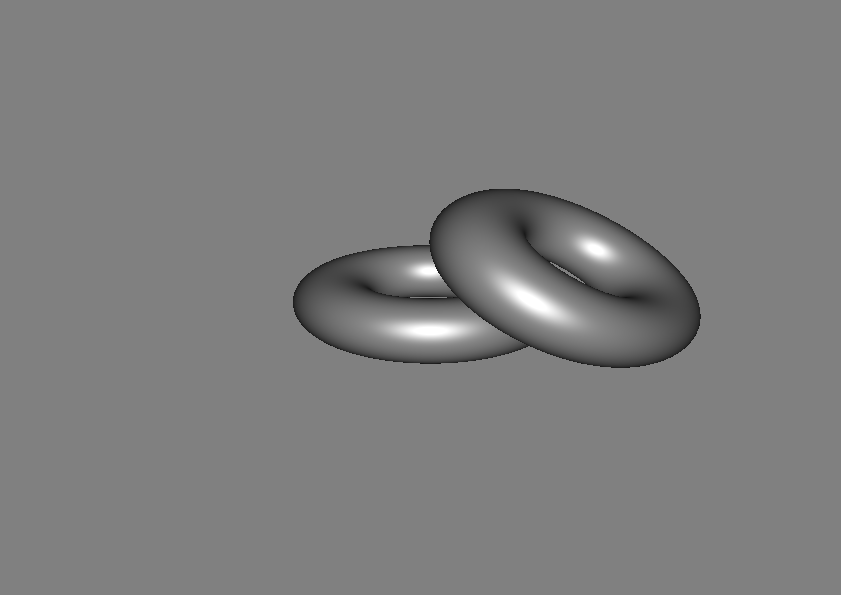
\includegraphics[width=.8\linewidth]{gauche.png}
  \caption{Prise de vue correspondant à la vue gauche}
\end{subfigure}%
\begin{subfigure}{.5\textwidth}
  \centering
  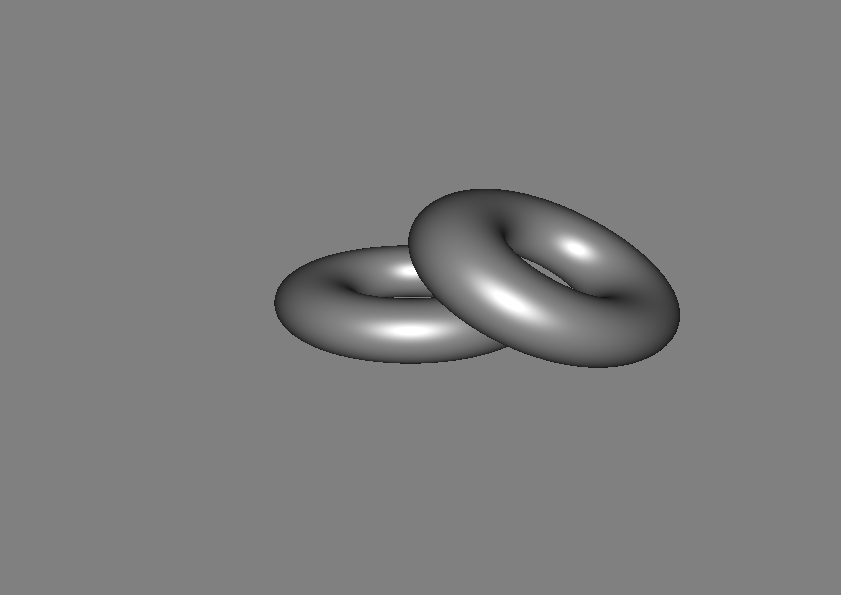
\includegraphics[width=.8\linewidth]{droite.png}
  \caption{Prise de vue correspondant à la vue droite}
\end{subfigure}
\caption{Les deux prises de vue obtenues avec translation}
\end{figure}

	\end{frame}
%%------------------------------------------------
%
\begin{frame}
\frametitle{Anaglyphe (2/6)}
\begin{itemize}[label=$\bullet$]
\item Méthode Photoshop \cite{stereoAnaglyph}
	\begin{itemize}[label=$\circ$]
	\item Deuxième étape : extraction du canal rouge pour la vue gauche, canaux verts et bleus pour la vue droite 
	\end{itemize}
\end{itemize}
\begin{figure}
\centering
\begin{subfigure}{.5\textwidth}
  \centering
  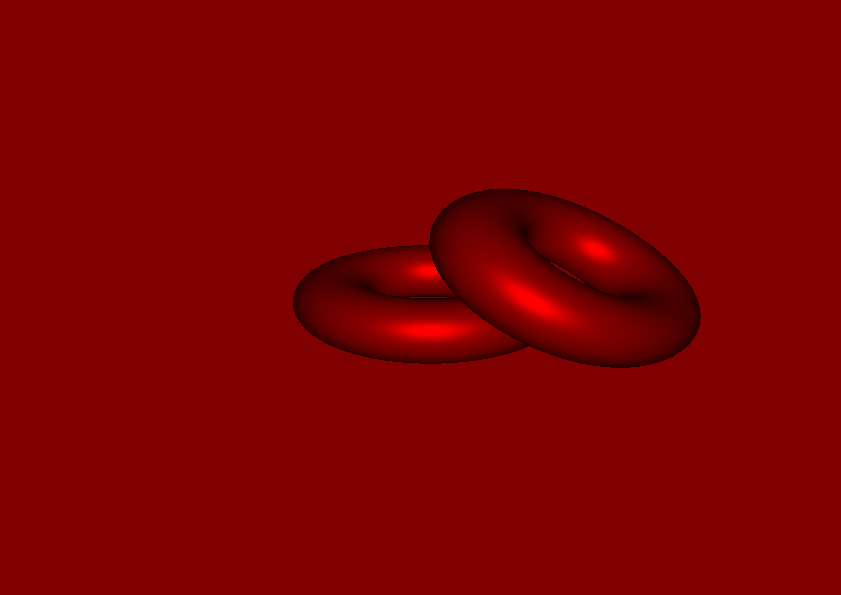
\includegraphics[width=.8\linewidth]{gauche_rouge.png}
  \caption{Vue gauche avec extraction du canal rouge}
\end{subfigure}%
\begin{subfigure}{.5\textwidth}
  \centering
  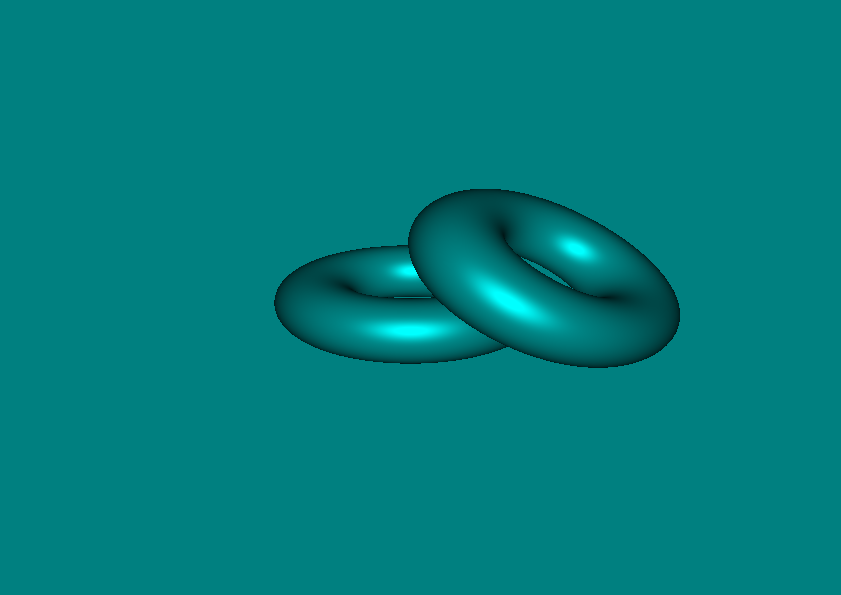
\includegraphics[width=.8\linewidth]{droite_cyan.png}
  \caption{Vue droite avec extraction des canaux bleu et vert}
\end{subfigure}
\caption{Les deux vues rouge et cyan}
\end{figure}


	\end{frame}

%%------------------------------------------------
%
\begin{frame}
\frametitle{Anaglyphe (3/6)}
\begin{itemize}[label=$\bullet$]
\item Méthode Photoshop \cite{stereoAnaglyph}
	\begin{itemize}[label=$\circ$]
	\item Troisième étape : composition de l'image à partir des canaux RGB des deux images
	\item Méthode efficace pour des objets simples ayant peu de détails
	\end{itemize}
\end{itemize}
\begin{figure}
\centering
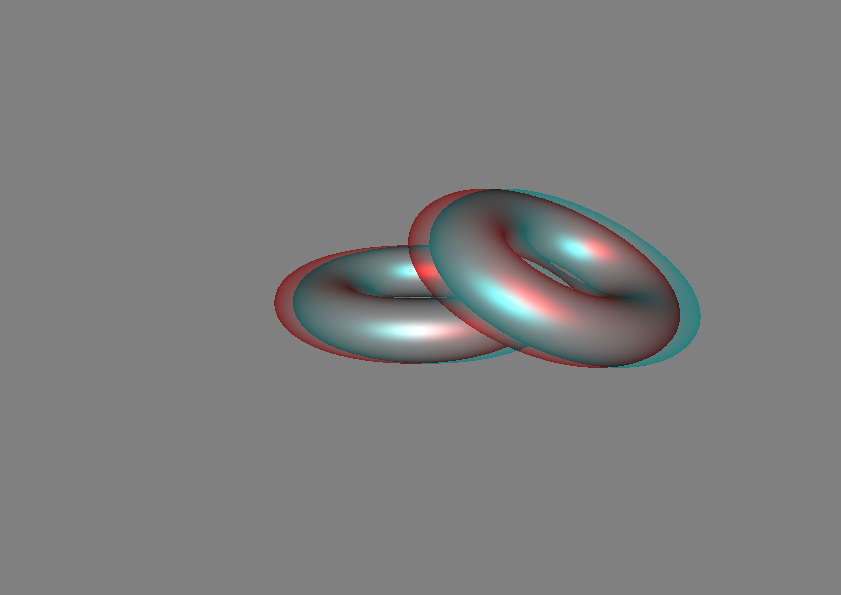
\includegraphics[scale=0.28]{donuts_photoshop.png}
\caption{Anaglyphe avec la méthode Photoshop d'un objet simple ayant peu de détails }
\end{figure}


\end{frame}


%%------------------------------------------------
%
\begin{frame}
\frametitle{Anaglyphe (4/6)}
\begin{itemize}[label=$\bullet$]
\item Méthode Photoshop \cite{stereoAnaglyph}
	\begin{itemize}[label=$\circ$]
	\item Méthode moins efficace pour les objets complexes 
	\item Plusieurs artefacts visibles
	\item Les détails ne sont pas soignés
	\end{itemize}
\begin{figure}
\centering
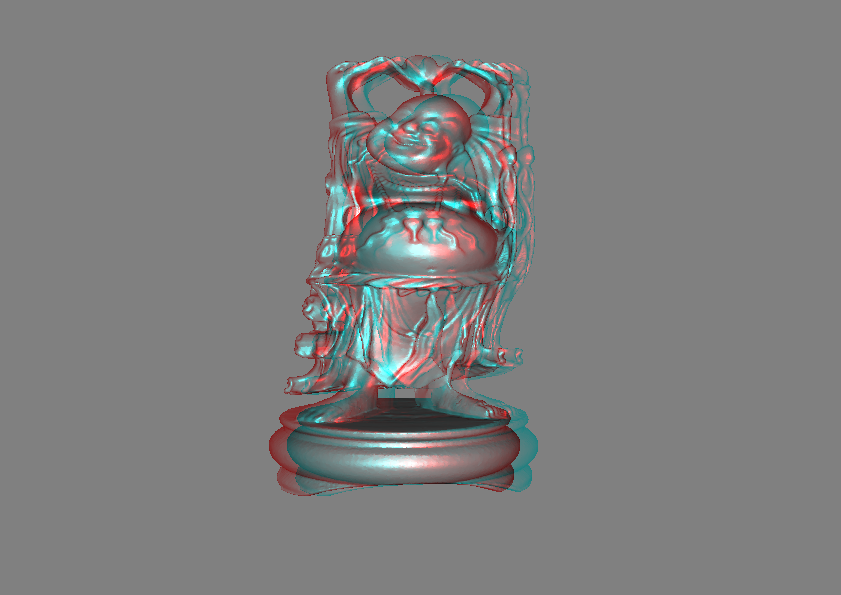
\includegraphics[scale=0.3]{happy_photoshop.png}
\caption{Anaglyphe avec la méthode Photoshop d'un objet complexe ayant beaucoup de détails }
\end{figure}
	
\end{itemize}

\end{frame}
% TODO : rajouter slide : mettre pour happy avec photoshop : marche moins bien 

%%------------------------------------------------
%
% ORAL : on a continué notre recherche
% les vraies deux images décalées
\begin{frame}
\frametitle{Anaglyphe (5/6)}
\begin{itemize}[label=$\bullet$]
\item Méthode Dubois \cite{algoDubois}
	\begin{itemize}[label=$\circ$]
	\item Combinaison de couleurs plus élaborée
	\item Conservation des détails de l'objet dans l'anaglyphe 
	\end{itemize}
\end{itemize}
\begin{figure}
\centering
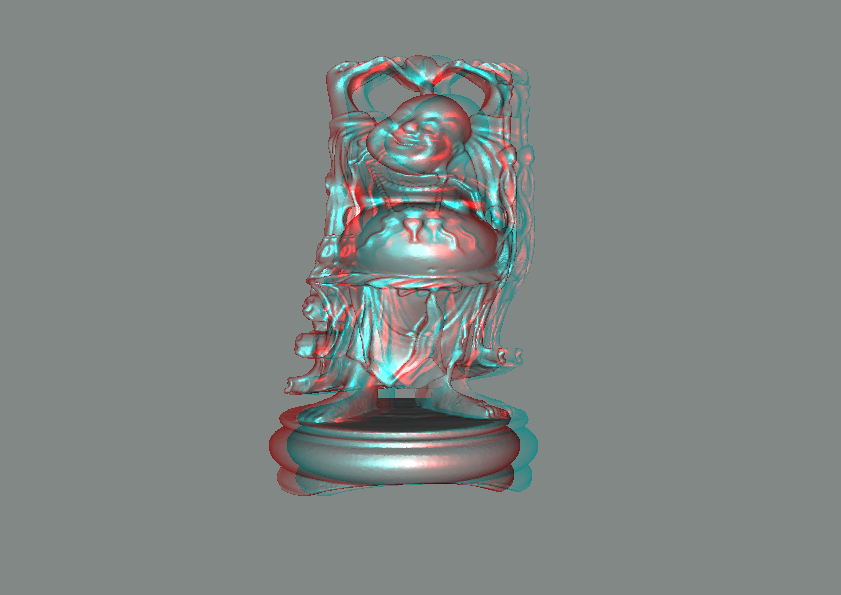
\includegraphics[scale=0.3]{happy_dubois.png}
\caption{Anaglyphe avec l'algorithme de Dubois d'un objet complexe ayant beaucoup de détails}
\end{figure}

\end{frame}

%%------------------------------------------------
%
% 
\begin{frame}
\frametitle{Anaglyphe (6/6)}
\begin{itemize}[label=$\bullet$]
\item Méthode Dubois \cite{algoDubois}
	\begin{itemize}[label=$\circ$]
	\item Légèrement moins efficace pour les objets simples 
	\end{itemize}
\end{itemize}
\begin{figure}
\centering
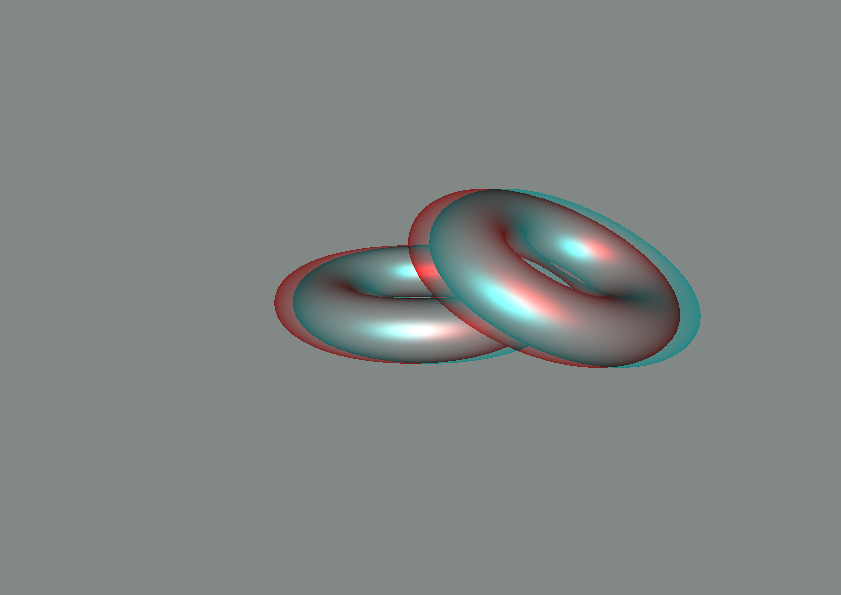
\includegraphics[scale=0.35]{donuts_dubois.png}
\caption{Anaglyphe avec l'algorithme de Dubois d'un objet simple avec peu de détails}
\end{figure}
\end{frame}
%------------------------------------------------

\begin{frame}
\frametitle{Besoins non fonctionnels - Portabilité}
\begin{itemize}[label=$\bullet$]
 	\item Linux
 	\begin{itemize}[label=$\checkmark$]
	\item Debian Jessie (64bits)
	\item Fedora 21 (64bits)
	\item ArchLinux (64bits)
	\end{itemize}
	\item Windows
	\begin{itemize}[label=$\checkmark$]
	\item Windows 7 (64bits)
	\item Windows 8 (64bits)
	\end{itemize}
\end{itemize}

\end{frame}

%%------------------------------------------------%

\begin{frame}
\frametitle{Besoins non fonctionnels - Fluidité}
\begin{itemize}[label=$\bullet$]
\item Résultats obtenus avec la version finale du logiciel
\end{itemize}
{\fontsize{7}{8}\selectfont
\arrayrulecolor{black}
\begin{tabular}{lccc}

\textbf{Carte Graphique} & \textbf{fps} & \textbf{Nombre de points souhaités}& \textbf{Nombre de points réels}\\
\\
\hline
\\
Intel HD Graphics 4000 &
20 & 150 000 &  1 630 000\\
\hline
\\
Intel HD Graphics 4000 &
25 & 
100 000 & 1 050 000 \\
\hline
\\
NVidia GeForce GTX 770 & 20 & 500 000 & 8 150 000\\
\hline
\\
NVidia GeForce GTX 770 & 25 &
350 000 & 7 600 000\\

\end{tabular}
}

\end{frame}

%------------------------------------------------

\begin{frame}
\frametitle{Bilan technique}
\begin{itemize}[label=$\bullet$]
\item Besoins fonctionnels
	\begin{itemize}[label=$\checkmark$]
	\item Manipulation de la scène
	\item Manipulation des objets
	\item Sauvegarde et chargement
	\item Anaglyphes, autostéréogrammes, folioscopes
	\end{itemize}
\item Besoins non fonctionnels
	\begin{itemize}[label=$\checkmark$]
	\item Extensibilité
	\item Portabilité  
	\item Fluidité
	\end{itemize}
\end{itemize}

\end{frame}

%%------------------------------------------------%

\begin{frame}
\frametitle{Difficultés rencontrées}
\begin{itemize}[label=$\bullet$]
\item Difficultés techniques
\begin{itemize}[label=$\circ$]
\item Utilisation des shaders
\item Portabilité Windows/Linux
\end{itemize}
\item Difficultés d'implémentations
\begin{itemize}[label=$\circ$]
\item Choix des algorithmes
\item Compréhension et implémentation
\end{itemize}
\end{itemize}

\begin{figure}
\centering
\begin{subfigure}{.4\textwidth}
  \centering
  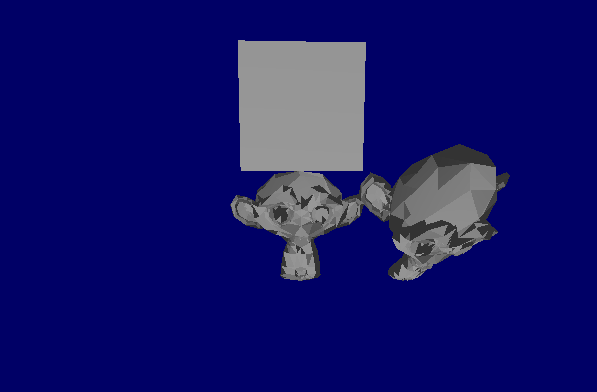
\includegraphics[width=1\linewidth]{rendu_sans_shader.png}
  \caption{Rendu sans shaders}
\end{subfigure}
\begin{subfigure}{.4\textwidth}
  \centering
  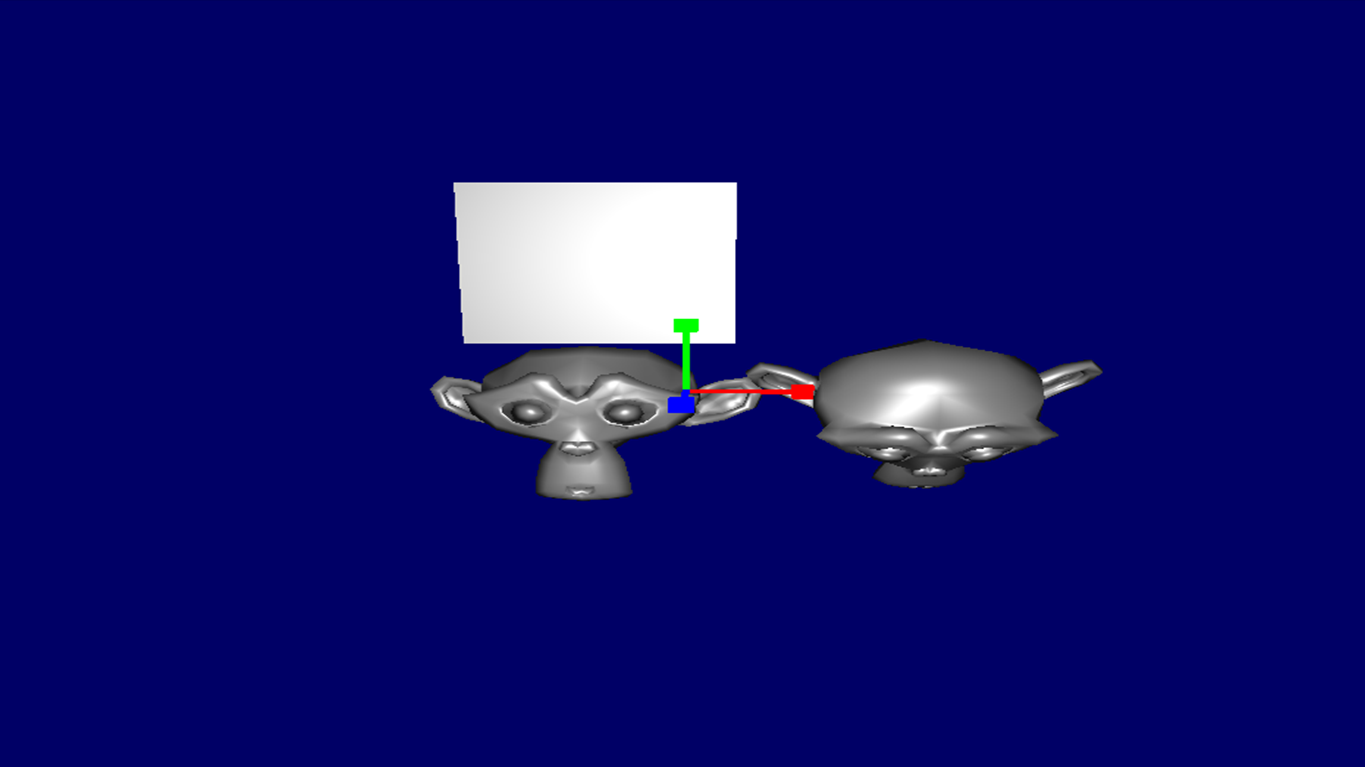
\includegraphics[width=1\linewidth]{singe_shaders.png}
  \caption{Rendu avec shaders}
\end{subfigure}
\caption{Comparaison de rendu avec ou sans shaders}
\end{figure}


\end{frame}

%------------------------------------------------
\section{Gestion de projet}

\begin{frame}
\frametitle{Déroulement du projet}
\begin{itemize}[label=$\bullet$]
\item Réalisation du cahier des charges
	\begin{itemize}[label=$\circ$]
	\item Rigueur de la rédaction
	\end{itemize}
\item Implémentation du logiciel
	\begin{itemize}[label=$\circ$]
	\item Répartition de l'équipe
	\item Utilisation des créneaux pour les réunions
	\end{itemize}
\end{itemize}

\end{frame}

%------------------------------------------------

\begin{frame}
\frametitle{Réalisation du diagramme de Gantt}
{\fontsize{7}{8}\selectfont
\arrayrulecolor{black}
\begin{tabular}{lcr}

\textbf{Tâche} & \textbf{Durée Prévisionnelle} & \textbf{Durée réelle} \\
\\
\hline
\\
Génération des flipbooks & 2semaines & 2 semaines \\
\hline
\\
Insertion de plusieurs objets \\ dans une scène &
3 semaines en fin de projet & 
1 semaine et demie \\ inclus dans 
une autre tâche \\ en début de projet \\
\hline
\\
Sauvegarde et chargement & 2 semaines puis 3 semaines &
7 semaines dont 4 effectives \\
\hline
\\
Prise de décision pour les shaders & X & 3 semaines\\
Recherche et implémentation \\des algorithmes &
4 semaines & 13 semaines \\
\hline
\\

\end{tabular}
}

\end{frame}

%------------------------------------------------

\begin{frame}
\frametitle{Apports et difficultés}
\begin{itemize}[label=$\bullet$]
\item Apports de ce projet
	\begin{itemize}[label=$\circ$]
	\item Projet de taille importante et équipe nombreuse
	\item Suivi régulier du client
	\end{itemize}
\item Quelques difficultés rencontrées
	\begin{itemize}[label=$\circ$]
	\item Appréciation de la durée des tâches
	\item Gestion d'équipe
	\end{itemize}
\end{itemize}

\end{frame}

%%------------------------------------------------
%
% faire une transition pour la bliblioraphie
\frame[allowframebreaks]{\frametitle{Bibliographie}
	\bibliographystyle{unsrtnat}
	\bibliography{bibli}
		
	}
	
%------------------------------------------------
	% juste dire à l'oral merci pour votre attention
	% TODO : annuler le style de cette slide et laisse l'image en grand 
\begin{frame} 
\begin{figure}
\hspace*{-1cm}
\centering
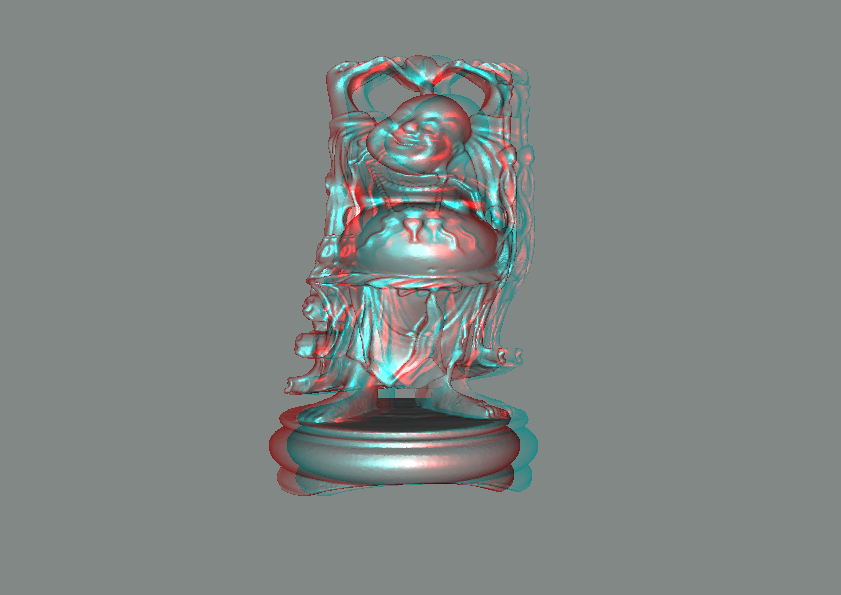
\includegraphics[scale=0.6]{happy_dubois.png}
\end{figure}

\end{frame}

%----------------------------------------------------------------------------------------

\end{document} 
